\documentclass[a4paper, article, english, oneside, unknownkeysallowed, 12pt]{memoir} 
\usepackage{preamble}


\usepackage[
  backend=biber,
  style=authoryear-ibid,
  maxcitenames=2,  % show up to 2 authors in citations
  mincitenames=1,  % use "et al." if more than 2
  maxbibnames=10,  % show up to 10 names in bibliography
  minbibnames=1,
    uniquelist=false,
    uniquename=false
]{biblatex}


\addbibresource{causal_effect_schools.bib}

\AtEveryBibitem{%
  \clearfield{urlyear}%
  \clearfield{urlmonth}%
  \clearfield{urlday}%
  \clearfield{urldate}%
}

% Name and Title
\title{Causal effects of schools on higher education outcomes - Spring update}
\author{ Bruno E. Aravena-Magüida}
\date{April 2026}

% Header (top) and footer (bottom)
\pagestyle{fancy}
\fancyhead[R]{\emph{3rd-year micro group}}
 \fancyhead[L]{BEAM} % keep section names
\fancyfoot[R]{}
\fancyfoot[L]{}


\begin{document}

% Prints title block from macros given above
\maketitle

% Prints a table of contents
\setcounter{tocdepth}{2}
\renewcommand\contentsname{}
%\tableofcontents* 
%\clearpage

\section{Introduction}

In this report, I present the progress I have made in the last month. I will go over the intuition behind the main changes in my approach and the current methodology I am using.
I will show some results and briefly discuss their interpretation.


\section{From school-specific effects to a scalar school-value treatment.}

My original intent of this paper was to measure idiosyncratic effects of each school on higher education outcomes.
The main challenge I was facing as a result, was that of having many unordered treatments -- one per high school and the absence of a clear control group.
The school assignment system is designed to give all students a school\footnote{no student is left unassigned: if unlucky in the first round students are assigned a spot in their original schools, and a complementary round matches students to the closest available spot at the end}. Even if some students drop out (and we ignore selection into that), we would need individuals dropping out on each `randomization cluster'.

As an example, suppose a mass of students with identical preferences for 3 schools, say $A \succ B \succ C$, and identical priority levels. 
Suppose furthermore, that all of them have guaranteed admission to school $G$ once the spots have run out for these three schools. 
Because we could compare the outcome of each school relative to the guaranteed admission school $G$, we could estimate the effect of each school relative to $G$.   

We could construct something like $\beta_{AG}, \beta_{BG}, \beta_{CG}$, where $\beta_{AG}$ would be the effect of attending school $A$ relative to $G$, and so on.
Given the common comparison group, we could even go further and call these effects $\beta_{A}, \beta_{B}, \beta_{C}$, and even rank them (e.g.  $\beta_{A} > \beta_{B} > \beta_{C} \implies A > B > C$) as they would be comparable across schools.

Suppose now that these students have guaranteed admission to different schools, say $G = (G^1, G^2, ..., G^{10})$. 
Note now that we would need to estimate 30 objects ($\beta_{AG^1}, \beta_{AG^2}, ..., \beta_{CG^{10}}$) and that we would not be able to rank them as they are not comparable across schools, except for comparisons within the same guaranteed admission school.
In this case, we would not be able to say anything about the relative ranking of schools \(A\), \(B\), and \(C\).


One solution to this problem is to collapse some of these treatment options. For instance, collapse guaranteed admission schools into two buckets, 
and define $\tilde{G} = (G^L, G^H)$. An example of something similar is \textcite{kirkeboen_field_2016}, which studies the causal effect of different higher education programs on labor market outcomes.
Given that they use a centralized assignment mechanism for higher education in Norway, their instrument is the score cutoff for each program. 
Given that people have different lists, they have different fallback options. Instead of estimating all the program effects relative to each other, they collapse the programs only into 10 fields and estimate 90 next-best effects. 
Note that to collapse the treatment options, they abstract away from differences in institutional quality in their main specification.


\begin{figure}[htbp]
\centering
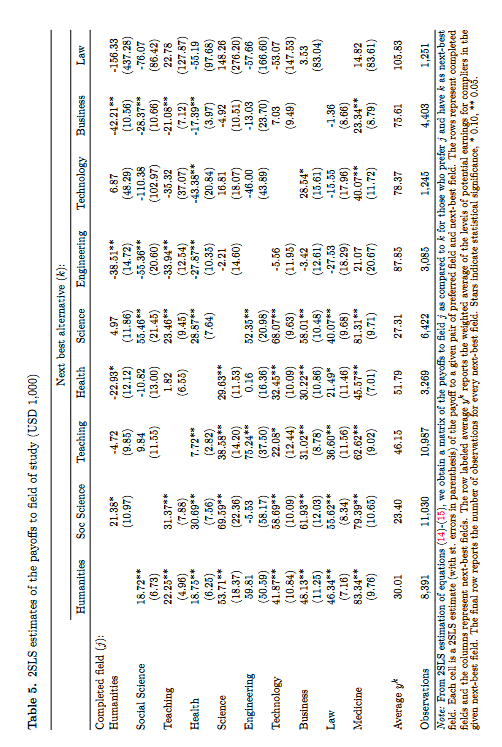
\includegraphics[width=0.75\textwidth,  angle=270]{magne_table.png}
\caption{Effect of payoffs of different fields of study relative to their next-best alternative. Source: \textcite{kirkeboen_field_2016}.}
\label{fig:main_result}
\end{figure}

My original concern with doing something like this in my paper was my intention to use this paper to identify whether specific schools were overperforming their peer institutions on some outcomes, as opposed to asking if some group of schools were overperforming others.

Talking to Prof. Walters was especially helpful in realizing that instead of collapsing schools on a categorical variable, I could do so on a continuous one. 
More importantly, the continuous variable can be constructed in a way that preserves the idiosyncratic effects of each school, while also allowing for comparability across schools.

Going back to our original example, if we have a metric $V$ for each of the schools (e.g. $V(A) = 3, V(B) = 5, V(C) = 7, V(G^i) = i$) then we can pool over multiple comparisons. 
Outcome differences between $A$ relative to $G^1$ (a gain of 2 in the V metric) would be comparable to outcome differences between $B$ relative to $G^3$ (also a gain of 2 in the V metric), and so on.
This way, we can estimate a single parameter $\theta$ that captures the effect of attending a school with a higher V metric relative to attending a school with a lower V metric. 

In particular, I will construct these V metrics using the observational value-added of each school on a particular outcome. 
I will then answer the question whether movements in a particular metric induced by the lottery offers, are correlated with differences in outcomes.
Given that the lottery offers encode exogenous variation we can interpret the results causally. 


\section{Methodology}
  \subsection{Computing Observational Value-Added for each school}

To compute observational value-added for each school, I use the universe of students who ever attended grade 8 in the Chilean education system between 2017 and 2020, defining their cohort by the first year they show up in grade 8 in this period.
 This corresponds to roughly 945,000 unique individuals. I track their performance in national mathematics and verbal achievement exams \textit{(SIMCE)} (grade 4 for all, grade 8 for some). I have demograhpic controls such as gender, their age at grade 8, and their commune. 
 I consider the 4 years after a student shows up in grade 8, and define their high school attended by institution attended the longest, prioirtizing the most recent in case of ties. For outcomes, I currently focus in achievement in a standarized higher-education entrace exams \textit{(PSU/PAES)} in both verbal and mathematics, as well as enrolmment into a STEM program. 



Following the value-added literature \parencite{chetty_measuring_2014,angrist_leveraging_2017}, I run a regression of the following form to compute the observational value-added for each school for each of these outcomes:
\[ Y_i = \mu + \beta_{S_i}  + \sum_{p=1}^{3} \lambda_{Mp} M_i^p + \sum_{p=1}^{3} \lambda_{Lp} L_i^p 
+ \gamma_{\mathrm{cohort}(i)} + \delta_{\mathrm{gender}(i)} + \rho_{\mathrm{age}(i)} + \kappa_{\mathrm{comuna}(i)}
+ \varepsilon_i .
\]

where \(Y_i\) is the outcome for student \(i\), and \(S_i\) is the school attended by student \(i\), as defined above. The coefficient \(\beta_{S_i}\) is a school fixed effect. \(M_i\) and \(L_i\) are the student's standardized fourth-grade math and language scores, respectively, which enter as third-order polynomials. The terms \(\gamma_{\mathrm{cohort}(i)}\), \(\delta_{\mathrm{gender}(i)}\), \(\rho_{\mathrm{age}(i)}\), and \(\kappa_{\mathrm{comuna}(i)}\) are fixed effects for the student's grade-8 cohort, gender, grade-8 age, and home commune, respectively. The error term is \(\varepsilon_i\).

I also construct an unadjusted measure which corresponds to the raw school mean:
\[
\beta_s^{\mathrm{raw}} = \frac{1}{N_s}\sum_{i:S_i=s}Y_i.
\]

We can partially see the role of these adjustments in Figure \ref{fig:VA by region}.
Figure \ref{fig:VA by region} shows the average value-added for math scores and STEM enrollment by region, comparing the unadjusted and adjusted metrics. For instance, schools in the capital region (RM) have very high unadjusted VA metrics, but adding controls significantly lowers these estimates on average. This indicates that these student populations tend to be positively selected.


\begin{figure}[htbp]
\centering

\includegraphics[width=0.75\textwidth]{C:/Users/xd-br/Desktop/PhD/Research/causal_schools/output/figures/school_rbd_observational_values/math_values_by_region_raw_adjusted.png}
\caption{Average VA in math score and STEM enrollment, by region. Comparing unadjusted and adjusted metrics. }
\label{fig:VA by region}
\end{figure}


It is important to clarify that by no means I intend to claim that these value-added metrics are causal. I propose thinking of them as a (selection-contaminated) measure of the causal school effect. We will use the IV regression to determine how informative these are. 

  \subsection{IV Regression: Projecting lottery-induced variation into Value-Added}

Once we have the observational value-added for each school ($\beta_s$), I proceed as follows.

First, given the lottery design, I only have instruments for students who apply for a change of school in the centralized mechanism. 
More precisely, I reduce the IV estimation sample to students who participate in the grade-9 centralized assignment process on time and for whom the assignment-probability simulations imply non-trivial admission risk.

\subsubsection{Students with assignment risk}
I define a student as at (assignment) risk if the simulated assignment probabilities do not place all probability mass on a single option. Formally, student \(i\) is included only if
\[
\max_{s \in \mathcal{S}} p_{is} < 1,
\]
where \(p_{is}\) is the simulated probability that student \(i\) is assigned to school \(s\).

\subsubsection{School support}

To reduce the dimensionality of the assignment-probability controls, I restrict the supported lottery school set to schools that appear with positive simulated assignment probability for at least 100 at-risk students. Let
\[
N_s^{+}
=
\sum_i
\mathbf{1}\{p_{is} > 0\}
\]
among students in the at-risk lottery sample. The supported school set is
\[
\mathcal{S}^{100}
=
\left\{
s : N_s^{+} \geq 100
\right\}.
\]


While the number 100 is an arbitrary threshold, I present its relevance in Table~\ref{tab:student_shares_by_sae_support_thresholds}. 
Table~\ref{tab:student_shares_by_sae_support_thresholds} reports how students in the broad grade-8 universe are distributed across schools by whether their attended school belongs to the SAE support set under alternative support thresholds.
With the 100-student threshold, we can estimate the 2SLS for supported schools that span 52.3 \% of the broad grade-8 universe using roughly 2,000 assignment-probability controls (2 for each supported school: probability of assignment and an indicator for zero probability).
An intermediate 50-student threshold would increase coverage to 67.2 \% while increasing the supported set from 1,011 to 1,562 schools.

\textcite{angrist_leveraging_2017} uses a threshold of 25 in their paper, but their number of schools is much smaller (lower than 50). In my setting, a 25-student threshold would cover 76.2 \% of the broad grade-8 universe but would require controls for 1,972 supported schools. I intend to move in that direction, potentially through the 50-student threshold first, but estimation is currently very computationally intensive. 

\begin{table}[!htbp]
\centering
\caption{Student shares by SAE support threshold and school type}
\label{tab:student_shares_by_sae_support_thresholds}
\begin{tabular}{llrrr}
\toprule
Threshold students at risk & School group & Schools & Students & Share \\
\midrule
100 & SAE <100 & 1,491 & 315,261 & 33.4\% \\
100 & SAE >=100 & 1,011 & 493,955 & 52.3\% \\
100 & Particular Pagado & 497 & 87,373 & 9.3\% \\
100 & Other non-SAE schools & 1,134 & 47,771 & 5.1\% \\
\midrule
25 & SAE <25 & 530 & 89,266 & 9.5\% \\
25 & SAE >=25 & 1,972 & 719,950 & 76.2\% \\
25 & Particular Pagado & 497 & 87,373 & 9.3\% \\
25 & Other non-SAE schools & 1,134 & 47,771 & 5.1\% \\
\bottomrule
\end{tabular}
\end{table}



\subsubsection{2SLS Regression}




For each school-value measure \(\beta_s\), I assign to each student the value of the school they attend:
\[
D_i = \beta_{S_i}, 
\]
where \(S_i\) is the school attended by student \(i\). I instrument this attended-school value with the value of the school offered through the lottery:
\[
Z_i
=
\mathbf{1}\{O_i \in \mathcal{S}^{100}\}\beta_{O_i},
\]
where \(O_i\) is the school offered to student \(i\) in the first round of the centralized assignment process. Offers outside the supported set are assigned zero in the excluded instrument.

The 2SLS system is:
\[
D_i
=
\pi_0
+
\pi_1 Z_i
+
P_i'\psi_D
+
X_i'\lambda_D
+
u_i ,
\]
\[
Y_i
=
\alpha
+
\theta \widehat{D}_i
+
P_i'\psi_Y
+
X_i'\lambda_Y
+
\varepsilon_i .
\]

Where \(Y_i\) is the student outcome of interest, \(D_i\) is the observational value of the school attended by the student, and \(Z_i\) is the observational value of the school offered by the lottery. 
The vector \(P_i\) contains assignment-probability controls\footnote{As discussed above, it includes for each school $\in \mathcal{S}^{100}$ the probability of assignment and an indicator for whether the probability is zero.}, and \(X_i\) contains additional student-level controls. 
These are grade-8 cohort fixed effects, gender fixed effects, grade-8 age fixed effects, standardized fourth-grade math score, and standardized fourth-grade language score.
 The parameter of interest  \(\theta\) measures the causal effect of a lottery-induced increase in the observational school-value index.



\section{Preliminary Results}
  \subsection{Core Results}

\begin{table}[!htbp]
\centering
\caption{Scalar school-value IV estimates}
\label{tab:scalar_school_value_iv_main_results}
\begin{tabular}{lcccccc}
\toprule
 & \multicolumn{2}{c}{Math VA} & \multicolumn{2}{c}{Language VA} & \multicolumn{2}{c}{STEM VA} \\
\cmidrule(lr){2-3} \cmidrule(lr){4-5} \cmidrule(lr){6-7}
 & (1) & (2) & (3) & (4) & (5) & (6) \\
 & Unadjusted & Adjusted & Unadjusted & Adjusted & Unadjusted & Adjusted \\
\midrule
$\theta$ & 0.208 & 0.431 & 0.167 & 0.393 & 0.345 & 0.584 \\
SE & 0.033 & 0.057 & 0.032 & 0.062 & 0.046 & 0.068 \\
p-value & $<0.001$ & $<0.001$ & $<0.001$ & $<0.001$ & $<0.001$ & $<0.001$ \\
\midrule
First-stage coef. & 0.455 & 0.457 & 0.439 & 0.435 & 0.471 & 0.455 \\
First-stage SE & 0.007 & 0.008 & 0.006 & 0.006 & 0.006 & 0.006 \\
First-stage F & 4399.434 & 3656.108 & 5480.545 & 4899.106 & 6509.162 & 5086.449 \\
N & 105,902 & 105,893 & 105,902 & 105,894 & 135,588 & 135,588 \\
\bottomrule
\end{tabular}
\end{table}


Table~\ref{tab:scalar_school_value_iv_main_results} shows the results of the 2SLS regression above for each of the three outcome variables, comparing both the adjusted and unadjusted value-added metrics.

Interpretation of $\theta$ can be a bit tricky. The general interpretation is that a student induced by a lottery offer to attend a school (a complier) with a 1-unit higher value in the respective metric is expected to have a $\theta$-unit higher outcome.
So a student induced to attend a school with a 1 standard deviation higher value-added (adjusted) in math scores is expected to have a 0.431 standard deviation higher math score in the standardized test. 
Similarly, a student induced to attend a school with a 1 extra probability (adjusted) in STEM enrollment is expected to have a 0.584 higher probability of enrolling into a STEM program.

Given that the treatment and the outcome are in the same scale, we can also interpret $\theta$ as a measure of the predictive power of the value-added metric. \textcite{angrist_leveraging_2017} formalizes this and considers $\theta = 1$ as a test for the value-added metric being a perfect predictor of the causal effect of schools on the outcome.
This is equivalent to testing whether the conditions under which value-added recover a causal effect (e.g. selection -only- on observables) hold in this context.
Thus we expect metrics more correlated with the causal effects to have a higher $\theta$. This is what we see when we compare across the unadjusted and adjusted specification. Adjusted specifications have higher $\theta$ values and are closer to 1, as they are less prone to selection bias.


Overall, this allows us to conclude that the VA metrics (especially the adjusted ones) are predictive of lottery-induced causal effects across specifications. 
While these results are metric-specific, they also show that exogenous values in school assignments do change outcomes for individuals. 
To my knowledge, these are the first results to show that school assignment lotteries induce changes in higher education major choice, which is an important contribution in itself.

\subsection{STEM Enrollment results by gender}

\begin{table}[!htbp]
\centering
\caption{STEM enrollment scalar school-value IV estimates by gender}
\label{tab:scalar_school_value_iv_stem_gender_results}
\begin{tabular}{lcccccc}
\toprule
 & \multicolumn{3}{c}{STEM VA} & \multicolumn{3}{c}{STEM gender gap reduc. VA} \\
\cmidrule(lr){2-4} \cmidrule(lr){5-7}
 & (1) & (2) & (3) & (4) & (5) & (6) \\
 & All & Boys & Girls & All & Boys & Girls \\
\midrule
$\theta$ & 0.584 & 0.535 & 0.695 & -0.254 & -0.477 & 0.000 \\
SE & 0.068 & 0.088 & 0.097 & 0.078 & 0.122 & 0.087 \\
p-value & $<0.001$ & $<0.001$ & $<0.001$ & 0.001 & $<0.001$ & 0.998 \\
\midrule
First-stage coef. & 0.455 & 0.460 & 0.443 & 0.443 & 0.457 & 0.429 \\
First-stage SE & 0.006 & 0.008 & 0.010 & 0.006 & 0.009 & 0.009 \\
First-stage F & 5086.449 & 3197.971 & 2002.877 & 4954.448 & 2810.343 & 2154.287 \\
N & 135,588 & 67,221 & 68,367 & 125,672 & 63,669 & 62,003 \\
\bottomrule
\end{tabular}
\end{table}

The first 3 columns of table \ref{tab:scalar_school_value_iv_stem_gender_results} shows the results of the 2SLS regression for STEM enrollment in the complete IV sample, but also running regressions separately by gender. Note that column (1) matches column (6) in \ref{tab:scalar_school_value_iv_main_results}. 
Columns (2) and (3) suggests that schools with higher value-added in STEM enrollment are slightly more effective at increasing STEM enrollment for girls, although the difference is not statistically significant (p = 0.219). 
Columns (4) - (6) repeat this exercise, but instead of using the value-added metric in STEM enrollment they consider as value-added the female-male difference in STEM enrollment. Higher values imply relatively higher STEM enrollment rates for females. 
Through this projection, we identify schools that are better at closing the gender gap in STEM enrollment. However, we can see that in such schools the gap is closed through a reduction the probability of boys entering to STEM instead of inducing females to enter STEM. 

\subsection{Results by school funding differences}

\begin{table}[!htbp]
\centering
\caption{School funding per person scalar IV estimates, millions of 2021 pesos}
\label{tab:money_scalar_iv_results}
\begin{tabular}{lcccccc}
\toprule
 & \multicolumn{3}{c}{Funding per student} & \multicolumn{3}{c}{Growth in funding per student} \\
\cmidrule(lr){2-4} \cmidrule(lr){5-7}
 & (1) & (2) & (3) & (4) & (5) & (6) \\
 & Math & Language & STEM & Math & Language & STEM \\
\midrule
$\theta$ & -0.022 & -0.041 & 0.029 & -0.020 & -0.001 & 0.031 \\
SE & 0.027 & 0.028 & 0.014 & 0.048 & 0.050 & 0.021 \\
p-value & 0.416 & 0.144 & 0.042 & 0.685 & 0.979 & 0.132 \\
\midrule
First-stage coef. & 0.339 & 0.339 & 0.268 & 0.398 & 0.398 & 0.343 \\
First-stage SE & 0.039 & 0.039 & 0.037 & 0.034 & 0.034 & 0.030 \\
First-stage F & 73.554 & 73.554 & 53.356 & 139.699 & 139.699 & 127.650 \\
N & 97,303 & 97,303 & 123,953 & 96,501 & 96,501 & 123,052 \\
\bottomrule
\end{tabular}
\end{table}

Table \ref{tab:money_scalar_iv_results} shows the results of the 2SLS regression when we use as value-added metric the average per-student expenditure of each school (and the growth over time).
The results suggest that the expenditure-based metric is not predictive of lottery-induced causal effects on any of the specifications. It must be said that school funding in this set of schools is determined mostly by number of students attending.
As a result, the core of the funding per student should be mostly similar across schools. There are components which are not determined by the number of students. Some of these attempt to target specific populations, so interpretation is not straightforward. 


%\section{Extensions}
%  \subsection{Testing formally whether }
%  \subsection{Implement Empirical Bayes}


















\clearpage
\printbibliography

\end{document}










